%-----------------------------------------------------------------------------
%
%               Template for sigplanconf LaTeX Class
%
% Name:         sigplanconf-template.tex
%
% Purpose:      A template for sigplanconf.cls, which is a LaTeX 2e class
%               file for SIGPLAN conference proceedings.
%
% Guide:        Refer to "Author's Guide to the ACM SIGPLAN Class,"
%               sigplanconf-guide.pdf
%
% Author:       Paul C. Anagnostopoulos
%               Windfall Software
%               978 371-2316
%               paul@windfall.com
%
% Created:      15 February 2005
%
%-----------------------------------------------------------------------------


\documentclass[preprint]{sigplanconf}

% The following \documentclass options may be useful:

% preprint      Remove this option only once the paper is in final form.
% 10pt          To set in 10-point type instead of 9-point.
% 11pt          To set in 11-point type instead of 9-point.
% authoryear    To obtain author/year citation style instead of numeric.

\let\program\undefined % \program from acmtras2e conflicts with our program

\usepackage{amsmath}
\usepackage{program}
\usepackage{graphicx}

% hyphen-able fixed-width font
\newcommand{\ttt}[1]{{\texttt{\hyphenchar\font=`\-\relax #1}}}%`
\newcommand{\fixme}[1]{{\color{red} #1}}

\begin{document}

\special{papersize=8.5in,11in}
\setlength{\pdfpageheight}{\paperheight}
\setlength{\pdfpagewidth}{\paperwidth}

\conferenceinfo{Workshop on Programming Models for SIMD/Vector Processing - WPMVP'15}{February 7--8, 2015, San Francisco, CA, USA} 
\copyrightyear{2015} 
\copyrightdata{978-1-nnnn-nnnn-n/15/2} 
\doi{nnnnnnn.nnnnnnn}

% Uncomment one of the following two, if you are not going for the 
% traditional copyright transfer agreement.

%\exclusivelicense                % ACM gets exclusive license to publish, 
                                  % you retain copyright

%\permissiontopublish             % ACM gets nonexclusive license to publish
                                  % (paid open-access papers, 
                                  % short abstracts)

\titlebanner{DRAFT}        % These are ignored unless
\preprintfooter{SIMD in JavaScript via C++ and Emscripten}   % 'preprint' option specified.

\title{SIMD in JavaScript via C++ and Emscripten}
% \subtitle{Subtitle Text, if any}

\authorinfo{Peter Jensen}
           {Intel Corporation}
           {peter.jensen@intel.com}
\authorinfo{John McCutchan}
           {Google Inc.}
           {johnmccutchan@google.com}
\authorinfo{Ivan Jibaja}
           {Intel Corporation}
           {ivan.jibaja@intel.com}
\authorinfo{Dan Gohman}
           {Mozilla}
           {sunfish@mozilla.com}
\authorinfo{Ningxin Hu}
           {Intel Corporation}
           {ningxin.hu@intel.com}

\maketitle


%\category{CR-number}{subcategory}{third-level}

% general terms are not compulsory anymore, 
% you may leave them out
%\terms
%term1, term2

%\keywords
%keyword1, keyword2

\begin{abstract}

%problem
A recent trend in web development uses Emscripten, Mozilla's LLVM-to-JavaScript compiler, to port existing native C/C++ applications to the Web at near-native speeds. However, compute-intensive applications, such as games and media-processing, that make use of SIMD intrinsics or gcc style vector code are not able to be compiled into JavaScript.
%contribution 
This paper presents the use of Emscripten to generate JavaScript code from C++ programs that include such vector code by using JavaScript's SIMD.JS, a new portable SIMD language extension. SIMD.JS allows JavaScript programmers to exploit vector parallelism by using the provided SIMD primitives and operations in their compute-intensive applications. Emscripten will correctly translate a subset of available C++ SIMD x86 intrinsics into the corresponding operations defined in SIMD.JS
%result
Using Emscripten, we show that the SIMD.JS benchmarks can be automatically compiled from C++ into JavaScript using the Emscripten compiler and obtain an average of X.XX speedup, compared to a Y.YY speedup of the hand-generated benchmarks.  
%meaning
Emscripten's ability to generate fast vector code using the portable SIMD.JS language extension allows a new set of compute-intensive C/C++ applications to be ported to the web making full use of SIMD hardware.

\end{abstract}



\section{Introduction}

More computing is being performed in web browsers. Games, multimedia, 
image and video processing, and other compute-intensive applications are 
being ported to JavaScript to be made available on the Web. An increasingly 
popular approach for porting existing native applications to the web is to use
Mozilla's Emscripten LLVM-to-JavaScript compiler. Emscripten compiles
C/C++ code into highly optimizable JavaScript that runs at near-native speeds
without the use of any plugins.

While these applications can exploit the use of vector code when written in C/C++, 
JavaScript applications were not able to make full use of the high performant and 
energy efficient SIMD instructions which are now standard on modern x86 and 
ARM hardware from mobile to servers. With the recent introduction of the portable 
language extension SIMD.JS, JavaScript applications are now able to use the 
provided SIMD primitives and operations to improve its performance by making full 
use of the SIMD hardware available.

This paper explores the implementation and evaluation of Emscripten's ability to generate 
SIMD.JS code from its native C/C++ intrinsics counterpart. We present performance 
data of the SIMD.JS benchmarks in JavaScript that have been automatically generated
by Emscripten and compare it with its hand-written version. We use both of the 
available prototypes of the SIMD.JS language extension: Google's V8 and Mozilla's 
SpiderMonkey and show speedup in both.



\section{SIMD.JS}

SIMD is short for Single Instruction, Multiple Data.  It refers to CPU 
instruction level data parallelism.  Most modern CPUs have a significant 
portion of their available instructions dedicated to operating on data in
parallel.  Typically, those instructions will perform the same operation on 
elements in short vectors, e.g. vectors of length 4, 8, or 16.  Use of these 
instructions leads to increased performance, because more data processing is 
achieved with fewer instructions executed, and fewer instructions also means
power savings, which is of outmost importance on mobile battery powered
devices.  Figure~\ref{fig:simd} shows how four scalar additions are 
combined into a single operation.

\begin{figure}
\begin{center}
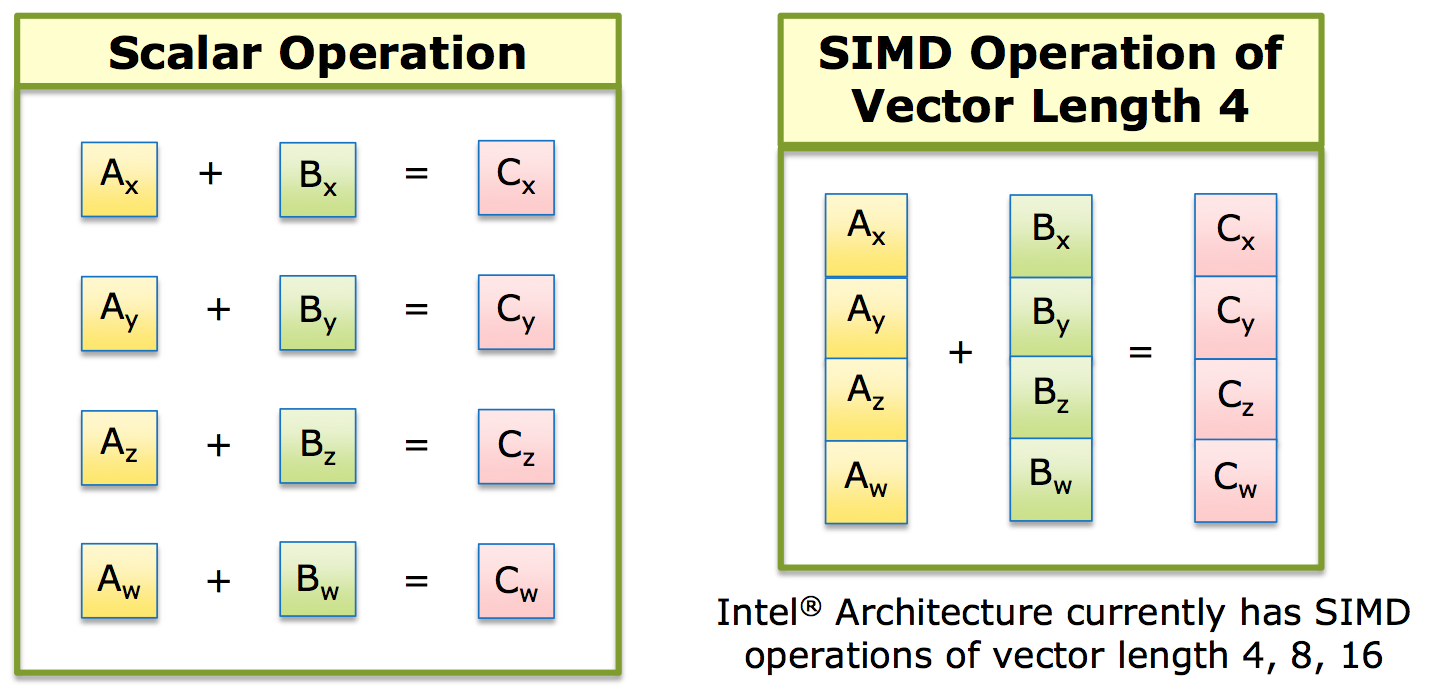
\includegraphics[width=0.45\textwidth]{figures/simd-04.png}
\end{center}
\caption{Replacing four scalar additions with one SIMD addition}
\label{fig:simd}
\end{figure}

JavaScript is quickly emerging as one of the most popular languages among 
software developers.  It was originally used for simple web page scripting for 
creating interactive web pages. Around 2008, very efficient and high 
performance JavaScript engines emerged, e.g. Firefox's TraceMonkey and 
Chrome's V8 engines. Since then, JavaScript has become a viable language for 
things beyond just basic web page interactivity, as witnessed by it's use in 
large web based applications, such as office applications; e-mail, document 
processing, etc. Also, large games, which were previously standalone, natively
compiled programs, have been ported to JavaScript to run within the browser 
environment.  More recently, JavaScript has been adopted as a server side 
scripting language (node.js), and lately, JavaScript has found it's way to the
mobil platform as a language that offers better portability between the 
different mobile platforms without sacrificing performance and features.  For 
example, access to platform sensors (location, accelerometers, etc) are 
accessible from JavaScript via W3C APIs.

Even with the past 7 years of JavaScript performance advances, the desire for 
better performing JavaScript engines has not lessened, quite the contrary. It's
a spiral that keeps on going; better performance leads to more uses, more uses 
require better performance.  Specifically, software that use data parallelism 
to achieve adequate performance have, so far, been restricted to natively 
compiled languages, such as C++, because such languages offer ways of utilizing 
the SIMD instructions available in modern CPUs.  JavaScript has only one number
type, Number, which is an IEEE-754 floating point number, and JavaScript offers 
no abstraction primitives for writing algorithms utilizing data paralellism, so 
it's imperative that this shortcoming is dealt with, such that the next leap
in JavaScript performance is made possible.  This is what the SIMD.JS proposal
addresses.

SIMD.JS is an emerging standard developed collaboratively by Intel, ARM,
Mozilla, Google, and Microsoft.  It provides low level data types and 
operations that map well onto the available SIMD instructions of the underlying 
hardware.  Currently, the defined data types and operations are a 
representative and useful overlap between SIMD types and operations available 
in most modern CPUs.

The SIMD.JS proposal is structured as an object hierarchy, with SIMD being the
top level global object.  The immediate properties of the SIMD object reflect
the data types; \ttt{int32x4}, \ttt{float32x4}, and \ttt{float64x2}.  The 
operations are methods declared as properties on the data type properties as 
outlined in  Figure~\ref{fig:hierarchy}, which shows a portion of the object 
hierarchy.

\begin{figure}
\begin{center}
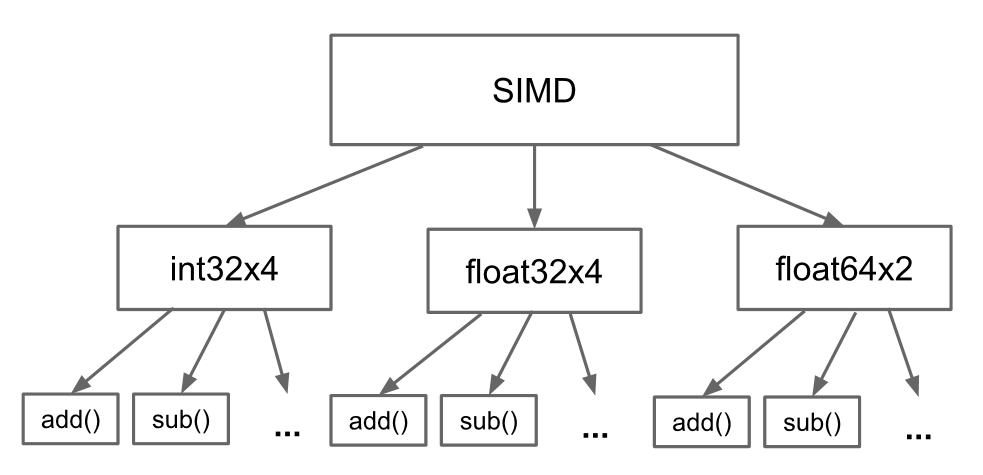
\includegraphics[width=0.45\textwidth]{figures/hierarchy.png}
\end{center}
\caption{SIMD.JS object hierarchy}
\label{fig:hierarchy}
\end{figure}

We've modelled the semantics of the SIMD types and operations as a polyfill 
<REF>.  This allows programmers to experiment without using a JavaScript
engine that natively supports SIMD.JS.  The polyfill also serves as documentation
for the semantics and interfaces.  It will also reflect the current state of
the proposal.  The proposal is under active development and changes are likely to 
happen as the proposal is being refined and moves forward through the approval
process.

As an example use case, Figure~\ref{fig:average-simd} shows the SIMD JavaScript
code for computing the average of an array of floating point numbers.  The numbers
are held in a Float32Array typed array; \ttt{data}.  The benefit of using SIMD 
operations, for computing the average, is that four numbers can be added in one
operation, thereby reducing the number of iterations by a factor of 4, and 
achieving an equivalent speedup.

\begin{figure}
\begin{small}
\begin{program}[style=tt, number=true]
fu\tab{}nction average(data) \{
  var sum = SIMD.float32x4.splat(0.0);
  fo\tab{}r (var i = 0, l = data.length; i < l; i = i+4) \{
    su\tab{}m = SIMD.float32x4.add(
      sum, SIMD.float32x4.load(data, i));\untab{}\untab{}
  \}
  var total = sum.x + sum.y + sum.z + sum.w;
  return total/data.length;\untab{}
\}
\end{program}
\end{small}
\caption{SIMD JavaScript code for finding the average of an array of numbers}
\label{fig:average-simd}
\end{figure}

\begin{figure}
\begin{small}
\begin{program}[style=tt, number=true]
371  cmp eax,edx
373  jnl 440  (270629B8)
379  cmp esp,[0x645e9c]
385  jc  445  (270629BD)
391  mov esi,eax
393  shl esi,1
396  add esi,0x10
399  mov ebx,ecx
401  shl ebx,1
404  cmp esi,ebx
406  ja  499  (270629F3)
412  movups xmm2,[edi+eax*2]
416  movaps xmm3,xmm1
419  addps xmm3,xmm2
422  mov ebx,eax
424  add ebx,0x8
427  jo  504  (270629F8)
433  movaps xmm1,xmm3
436  mov eax,ebx
438  jmp 371  (27062973)
\end{program}
\end{small}
\caption{JIT compiler generated code for the \ttt{for} loop in the \ttt{average} function}
\label{fig:average-simd-code}
\end{figure}

The optimizing Just-In-Time (JIT) compiler in our Chrome/V8 SIMD enabled
prototype is able to produce the code in Figure~\ref{fig:average-simd-code} for
the body of the loop.  The code shows how the compiler is able to utilize
128-bit SIMD registers (xmm) to hold the value of \ttt{sum} and to use the
\ttt{addps} instruction for adding 4 single precision numbers in one
instruction.  The details for this code snippet are as follows:

line 1-2: Check the loop index, \ttt{i}, against the upper bound and
exit the loop if upper bound is encountered.  \ttt{eax} holds the loop
index and \ttt{edx} holds the upper bound.

line 3-4: Check to enable the JavaScript engine to abort the
execution, if the loop has been running for too long.  It will prevent
a user program from hanging the browser.

line 5-11: Bounds check for the SIMD\_float32x4\_load operation. \ttt{eax}
holds the index and \ttt{ecx} holds the upper bound.

line 12: Load the 4 32-bit float values. \ttt{edi} holds the base address
of the data.  The reason the index is multiplied by 2 and not 4 is the fact
that V8 represents integers in bits 1-31, so the value in \ttt{eax} is already
holding the value of the index variable times 2.

line 13-14: Add the four 32-bit float values.

line 15-17: increment the loop index by 4.  Since the integer representation
used by V8 is done in bits 1-31 the actual value added is 8.  The overflow
checks is there to ensure that the result can still be represented in 31 bits,
if not the representation is switched to a boxed floating point number.

line 18: Move the result of the SIMD add operation, to the xmm1 register, which
holds the value of \ttt{sum}.

line 19-20: Move the new loop index value to it's proper register and jump back
to the top of the loop.

For more details on how the JIT compilers operate see <REF>.

\subsection{The Future of SIMD.JS}

The proposal has been presented to TC39, the JavaScript language standard
commitee, and was unanimously approved for stage 1 in 2014.  Stage 1 is the
proposal stage.  It indicates that the need has been justified, and an 
outline for a solution has been accepted.  It does not mean that this is the final
proposal.

The focus, so far, has been on identifying types and operations that can be
effectively implemented on all relevant CPU architectures.  We realize that CPUs
have destinct features that are useful and it will make sense to expose such 
features to the JavaScript programmer.  This will most likely be done via
architecture specific extensions to the SIMD object, e.g. SIMD.x86.*

SIMD.JS is currently being refined and prepared for the next stages of approval,
and we expect this to be part of the EcmaScript 7 standard (ES7).
EcmaScript 5 is the current JavaScript standard.  EcmaScript 6 is slated for a
mid-2015 release. ES6 is a major overhaul of the JavaScript language and a 
substantial set of new features were added, as reflected by the size of the 
language specification document.  The ES5 specification document is roughly 300 
pages, whereas the ES6 specification is roughly double that. Most browsers 
have already implemented most of the ES6 features.

\section{Emscripten}

Emscripten is a compiler that compiles C/C++ programs into JavaScript.  It is
based on the clang/LLVM compiler infrastructure <REF>.  The compiler is the
brainchild of Alon Zakai of Mozilla.

As an example of how it works, we'll look at the generated JavaScript code
resulting from compilign a simple C function.  We'll again use a function that
computes the average of float numbers.  Figure~\ref{fig:average-scalar} shows
the input C program.

\begin{figure}
\begin{small}
\begin{program}[style=tt, number=true]
fl\tab{}oat averageScalar(float *a, uint32\_t length) \{
  float  sum = 0.0f;
  fo\tab{}r (uint32\_t j = 0, l = length; j < l; j = j + 4) \{
    sum = sum + (*(a++));\untab{}
  \}
  return sum/length;\untab{}
\}
\end{program}
\end{small}
\caption{Scalar C code for the \ttt{average} function}
\label{fig:average-scalar}
\end{figure}

The Emscripten compiler command is similar to the clang compiler command, and
takes most of the same options.  The following command will generate optimized
JavaScript code shown in Figure~\ref{fig:average-scalar-code}:

\smallskip
\ttt{  \$ emcc -O2 -g average-scalar.c}
\smallskip

\begin{figure}
\begin{small}
\begin{program}[style=tt, number=true]
fu\tab{}nction \_averageScalar(\$a, \$length) \{
 \$a = \$a \textbar\ 0;
 \$length = \$length \textbar\ 0;
 var \tab{}\$a\$addr\$06 = 0, \$add = 0.0, \$j\$05 = 0,
     \$sum\$0\$lcssa = 0.0, \$sum\$04 = 0.0, sp = 0;\untab{}
 sp = STACKTOP;
 if\tab{} ((\$length \textbar\ 0) == 0)
   \$sum\$0\$lcssa = 0.0;\untab{}
 el\tab{}se \{
  \$a\$addr\$06 = \$a;
  \$j\$05 = 0;
  \$sum\$04 = 0.0;
  wh\tab{}ile (1) \{
   \$add = \$sum\$04 + +HEAPF32[\$a\$addr\$06 >> 2];
   \$j\$05 = \$j\$05 + 4 \textbar\ 0;
   if\tab{} (\!(\$j\$05 >>> 0 < \$length >>> 0)) \{
    \$sum\$0\$lcssa = \$add;
    break;\untab{}
   \}\tab{} else \{
    \$a\$addr\$06 = \$a\$addr\$06 + 4 \textbar\ 0;
    \$sum\$04 = \$add;\untab{}
   \}\untab{}
  \}\untab{}
 \}
 STACKTOP = sp;
 return +(\$sum\$0\$lcssa / +(\$length >>> 0));\untab{}
\}
\end{program}
\end{small}
\caption{JavaScript code generated by Emscripten for\newline the \ttt{averageScalar} function}
\label{fig:average-scalar-code}
\end{figure}

This example shows how Emscripten manages to map a staticly typed language (C) with pointers
to a dynamically typed language without pointers (JavaScript).

Memory is modelled as overlayed typed arrays.
In this example when the pointer \ttt{*a} is used to fetch from memory the corresponding
JavaScript code is \ttt{+HEAPF32[\$a\$addr\$06 >> 2]} (line 14).
\ttt{HEAPF32} is a global JavaScript typed array declared as follows:

\smallskip
\begin{program}[style=tt]
var buffer = new ArrayBuffer(TOTAL\_MEMORY);\newline
HEAP8 = new Int8Array(buffer);\newline
HEAP16 = new Int16Array(buffer);\newline
HEAP32 = new Int32Array(buffer);\newline
HEAPU8 = new Uint8Array(buffer);\newline
HEAPU16 = new Uint16Array(buffer);\newline
HEAPU32 = new Uint32Array(buffer);\newline
HEAPF32 = new Float32Array(buffer);\newline
HEAPF64 = new Float64Array(buffer);\newline
\end{program}
\smallskip

All of these typed arrays are views on the same array buffer, so they all
access the same physical memory.  Notice that the index expression
\ttt{'\$a\$addr\$06 >> 2'} is shifted right by 2.
This is because \ttt{\$a\$addr\$06} is a byte address, and elements in the
\ttt{HEAPF32} are 4 bytes each.

To enable the JavaScript JIT compilers to generate efficient code two
type coercision tricks are used.

For integers and pointers the \ttt{'expr \textbar\ 0'} is used to guarantee
that the type of the resulting expression is a 32-bit integer.  JavaScript
semantics of the the bitwise \textbar\ expression dictate that the resulting
expression is a 32-bit integer.  A side effect of pointers being 32-bit integers
is that compiled C/C++ programs are restricted to a 32-bit address space.

For floating point numbers, the unary '+' operator is applied, because JavaScript
semantics dictate that the resulting expression is a floating point number.

Emscripten has been successfully used to compiler very large C/C++ code
bases (+100K lines of code).  For example both Epic's and Unity's game engines
have been ported, using Emscripten <REF>.  Game engines are one example of
software that will have optional implementations of performance critical
portions of the code implemented using SIMD features.  Since, JavaScript
hasn't had a way of utilizing these powerful low level SIMD features of the
CPU, Emscripten has not been able to compile these highly tuned implementations
of the performance critical sections of the code. However, with the introduction
of SIMD.JS, Emscripten will now be able to take full advantage of those.  The next
section covers how this is accomplished.

\section{Compiling C++ with SIMD intrinsics}

Figure~\ref{fig:average-intrin} shows a typical SIMD implementation of the
\ttt{average} function in C, using x86 SIMD intrinsics.

\begin{figure}
\begin{small}
\begin{program}[style=tt, number=true]
fl\tab{}oat averageIntrin(float *a, uint32\_t length) \{
  \_\_m128 sumx4 = \_mm\_set\_ps1(0.0);
  fo\tab{}r (uint32\_t j = 0, l = length; j < l; j = j + 4) \{
    sumx4 = \_mm\_add\_ps(sumx4, \_mm\_loadu\_ps(a++)));\untab{}
  \}
  float mSumx4[4];
  \_mm\_storeu\_ps(mSumx4, sumx4);
  return (\tab{}mSumx4[0] + mSumx4[1] +
          mSumx4[2] + mSumx4[3])/length;\untab{}\untab{}
\}
\end{program}
\end{small}
\caption{SIMD C code with intrinsics for the \ttt{average} function}
\label{fig:average-intrin}
\end{figure}

The \ttt{\_\_m128} type holds 4 32-bit float numbers.  The \ttt{\_mm\_*\_ps}
function calls are the SIMD intrinsics, which operates on single precision 
\ttt{\_\_m128} values.  For example, the \ttt{\_mm\_add\_ps} intrinsic maps 
to the x86 \ttt{addps} instruction, which adds 4 32-bit float numbers in one 
operation.  This allows the iteration count to be reduced by a factor of 4
resulting in an equivalent speedup.

The resulting JavaScript produced by Emscripten is shown in
Figure~\ref{fig:average-intrin-js}.

\begin{figure}
\begin{small}
\begin{program}[style=tt, number=true]
fu\tab{}nction \_averageIntrin(\$a, \$length) \{
  \$a = \$a \textbar\ 0;
  \$length = \$length \textbar\ 0;
  var \tab{}\$add\$i = SIMD\_float32x4(0, 0, 0, 0),
      \$j\$09 = 0,
      \$sumx4\$0\$lcssa = SIMD\_float32x4(0, 0, 0, 0),
      \$sumx4\$010 = SIMD\_float32x4(0, 0, 0, 0),
      sp = 0;\untab{}
  sp = STACKTOP;
  if\tab{} ((\$length \textbar\ 0) == 0)
    \$sumx4\$0\$lcssa = SIMD\_float32x4\_splat(Math\_fround(0));\untab{}
  el\tab{}se \{
    \$j\$09 = 0;
    \$sumx4\$010 = SIMD\_float32x4\_splat(Math\_fround(0));
    whi\tab{}le (1) \{
      \$a\tab{}dd\$i =
        SI\tab{}MD\_float32x4\_add(
          \$sumx4\$010,
          SIMD\_float32x4\_load(buffer, \$a + (\$j\$09 << 2) \textbar\ 0));\untab{}\untab{}
      \$j\$09 = \$j\$09 + 4 \textbar\ 0;
      if\tab{} (\!(\$j\$09 >>> 0 < \$length >>> 0)) \{
        \$sumx4\$0\$lcssa = \$add\$i;
        break;\untab{}
      \} else \$sumx4\$010 = \$add\$i;\untab{}
    \}\untab{}
  \}
  STACKTOP = sp;
  return\tab{} +((+\$sumx4\$0\$lcssa.w + (+\$sumx4\$0\$lcssa.z +
        (+\$sumx4\$0\$lcssa.x + +\$sumx4\$0\$lcssa.y))) /
        +(\$length >>> 0));\untab{}\untab{}
\}
\end{program}
\end{small}
\caption{Emscripten generated SIMD JavaScript code for the \ttt{averageIntrin} function}
\label{fig:average-intrin-js}
\end{figure}

The JavaScript code in Figure~\ref{fig:average-intrin-js} might appear
extensive at first look, however, it is very similar to the handwritten
version of the function from Figure~\ref{fig:average-simd}.  The while loop
starting at line 15 corresponds to the for loop from the C program.  Implementing
a for loop as a while loop takes a bit more code.  The important thing to notice
here is the use of the \ttt{SIMD\_float32x4\_add} and \ttt{SIMD\_float32x4\_load}
SIMD.JS operations.  The use of '\_' instead of '.' is because Emscripten have
created single identifier versions for all the SIMD.JS primitives.

It's important to note that use of CPU specific intrinsics makes the C version
of the code target specific, i.e. it will only execute on x86 CPUs, whereas the
resulting JavaScript code will execute on all architectures supported by the
underlying SIMD enabled JavaScript engine.

Use of non target specific SIMD code in C is possible via the gcc
\ttt{vector\_size} attribute.  Emscripten also supports compiling such code.  A
non target specific version of the \ttt{average} function is shown in
Figure~\ref{fig:average-vector}.  The generated JavaScript code is virtually
identical to the code resulting from the C code using intrinsics. If
possible, developers should be encouraged to write their SIMD code using
this more universal syntax.

\begin{figure}
\begin{small}
\begin{program}[style=tt, number=true]
typedef float floatx4 \_\_attribute\_\_ ((vector\_size(16)));
fl\tab{}oat averageVectorSize(float *a, uint32\_t length) \{
  floatx4 sumx4 = \{0.0f, 0.0f, 0.0f, 0.0f\};
  floatx4 *ax4  = (floatx4 *)a;
  fo\tab{}r (uint32\_t j = 0, l = length; j < l; j = j + 4) \{
    sumx4 = sumx4 + *(ax4++);\untab{}
  \}
  return (\tab{}sumx4[0] + sumx4[1] +
          sumx4[2] + sumx4[3])/length;\untab{}\untab{}
\}
\end{program}
\end{small}
\caption{SIMD C code with \ttt{vector\_size} for the \ttt{average} function}
\label{fig:average-vector}
\end{figure}

\section{Benchmarks}

We've created a set of benchmark kernels.  The kernels are written in
both C++ and JavaScript.  Each kernel will have both a scalar implementation
and a SIMD implementation.

The C++ SIMD implementation is done using x86 intrinsics.  The C++ kernels are 
compiled with both the C++ clang compiler and with the Emscripten compiler.  
This gives us a basis for comparing SIMD/Scalar speedups for both C++ and
JavaScript as well as C++/JavaScript performance differences.  For the JavaScript
execution we've used our two SIMD enabled JavaScript engines; V8 and SpiderMonkey.

The benchmarks are written such that each kernel operation is executed as many times
as it takes for it to run in about a second.  This guarantees that the optimizing
JavaScript JIT compilers kick in, which is essential for optimimal performance.

The benchmark kernels we've collected performance data for are:

\begin{itemize}
\item
\textbf{AverageFloat32x4:} Average 10,000 32-bit float number.  This 
the kernel for the example used throughout the previous examples.

\item
\textbf{Mandelbrot:} Compute how many iterations it takes for
z(i+1) = z(i)**2 + c to diverge for seed point c = (0.01, 0.01).
Divergence is determined by z**2 \textgreater 4. This seed point never diverges, so
the loop always runs up to the maximum of iterations allowed.  The
maximum number of iterations for this kernel is set to 100.  The scalar version
of the kernel will compute the iteration count for one seed point, and
the SIMD version will compute the iteration count for four seedpoints.
As an example of how all the benchmark kernels are structured we've shown
the handwritten JavaScript and C++ version of this kernel in Figure~\ref{fig:mandel-js}
and Figure~\ref{fig:mandel-cpp}.

\item
\textbf{MatrixMultiplication:} Multiply two 4x4 matrices.  For each element in
the resulting 4x4 matrix, 4 scalar multiplications and 3 scalar additions are
required.  The SIMD version will rearrange the source data, using a shuffle operation,
and compute an entire row in the result matrix with 4 SIMD multiplies and 3 SIMD additions.

\item
\textbf{VertexTransform:} Multiply a 4x4 matrix with a 4 element vector.  This
is a common CPU side operation for creating projection matrices for webGL shaders.
Typically, it's used to compute a transformation for a point in 3D space, e.g. rotation
around an axis.  For each element in the resulting 4 element vector, 4 scalar multiplies
and 3 scalar additions must be computed.  The SIMD version will compute all 4 elements,
using SIMD multiplies and adds, thereby reducing the number of multiply and add instructions.
Some shuffling is required to get the input data into the right lanes.

\item
\textbf{MatrixTranspose:} Transpose a 4x4 matrix.  This is also a common operation, when
doing vector/matrix algebra.  Rows are made into columns.  The scalar kernel, simply moves
the 16 elements around one by one.  The SIMD version uses 8 shuffle operations.

\item
\textbf{MatrixInverse:} Compute the inverse of a 4x4 matrix.  This is a complex operation,
involving hundreds of multiples and add operations.  There are several different ways
of computing the inverse of a matrix.  Here we have chosen a method called the Cramer rule
<REF>.  This kernel is the most compute intensive.

\end{itemize}

\begin{figure}
\begin{small}
\begin{program}[style=tt, number=true]
\_\_\tab{}m128i mandelx4(\tab{}\_\_m128 c\_re4, \_\_m128 c\_im4,
                uint32\_t max\_iterations) \{\untab{}
  \_\_m128  z\_re4  = c\_re4;
  \_\_m128  z\_im4  = c\_im4;
  \_\_m128  four4  = \_mm\_set\_ps1(4.0f);
  \_\_m128  two4   = \_mm\_set\_ps1(2.0f);
  \_\_m128i count4 = \_mm\_set1\_epi32(0);
  \_\_m128i one4   = \_mm\_set1\_epi32(1);
  uint32\_t i;
  fo\tab{}r (i = 0; i < max\_iterations; ++i) \{
    \_\_m128 z\_re24 = \_mm\_mul\_ps(z\_re4, z\_re4);
    \_\_m128 z\_im24 = \_mm\_mul\_ps(z\_im4, z\_im4);
    \_\_\tab{}m128 mi4      =
      \_mm\_cmple\_ps(\_mm\_add\_ps(z\_re24, z\_im24), four4);\untab{}
    if\tab{} (\_mm\_movemask\_ps(mi4) == 0)
      break;\untab{}
    \_\_m128 new\_re4 = \_mm\_sub\_ps(z\_re24, z\_im24);
    \_\_m128 new\_im4 = \_mm\_mul\_ps(\_mm\_mul\_ps(two4, z\_re4), z\_im4);
    z\_re4 = \_mm\_add\_ps(c\_re4, new\_re4);
    z\_im4 = \_mm\_add\_ps(c\_im4, new\_im4);
    co\tab{}unt4 = \_mm\_add\_epi32(
      count4, \_mm\_and\_si128(\_mm\_castps\_si128(mi4), one4));\untab{}\untab{}
  \}
  return count4;\untab{}
\};
\end{program}
\end{small}
\caption{C++ SIMD Mandelbrot kernel}
\label{fig:mandel-cpp}
\end{figure}

\begin{figure}
\begin{small}
\begin{program}[style=tt, number=true]
fu\tab{}nction mandelx4(c\_re4, c\_im4, max\_iterations) \{
  var z\_re4  = c\_re4;
  var z\_im4  = c\_im4;
  var four4  = SIMD.float32x4.splat(4.0);
  var two4   = SIMD.float32x4.splat(2.0);
  var count4 = SIMD.int32x4.splat(0);
  var one4   = SIMD.int32x4.splat(1);
  fo\tab{}r (var i = 0; i < max\_iterations; ++i) \{
    var z\_re24 = SIMD.float32x4.mul(z\_re4, z\_re4);
    var z\_im24 = SIMD.float32x4.mul(z\_im4, z\_im4);
    var mi4    = SI\tab{}MD.float32x4.lessThanOrEqual(
                   SIMD.float32x4.add(z\_re24, z\_im24), four4);\untab{}
    // check if all 4 values are greater than 4.0
    if\tab{} (mi4.signMask === 0x00)
      break;\untab{}

    var new\_re4 = SIMD.float32x4.sub(z\_re24, z\_im24);
    va\tab{}r new\_im4 = SIMD.float32x4.mul(
      SIMD.float32x4.mul(two4, z\_re4), z\_im4);\untab{}
    z\_re4       = SIMD.float32x4.add(c\_re4, new\_re4);
    z\_im4       = SIMD.float32x4.add(c\_im4, new\_im4);
    co\tab{}unt4      = SIMD.int32x4.add(
      count4, SIMD.int32x4.and (mi4, one4));\untab{}\untab{}
  \}
  return count4;\untab{}
\}
\end{program}
\end{small}
\caption{JavaScript SIMD Mandelbrot kernel}
\label{fig:mandel-js}
\end{figure}

The sources for the C++ benchmarks can be found here: <REF>, and the sources
for the handwritten JavaScript benchmarks can be found here: <REF>

\section{Results}

We've collected performance results for these combinations:

\begin{itemize}
\item
Natively compiled C++

\item
Handwritten JavaScript executed with V8

\item
Emscripten produced JavaScript from C++ implementation executed with V8

\item
Emscripten produced JavaScript from C++ implementation executed with
SpiderMonkey
\end{itemize}

Note, we're not yet able to run 'generic'/handwritten SIMD JavaScript code
efficiently with SpiderMonkey.  SpiderMonkey uses two different JIT compilers;
one for 'generic' JavaScript code (IonMonkey) and another for the asm.js
JavaScript subset (OdinMonkey).  Only the OdinMonkey JIT compiler has been
adapted to work with the SIMD operations.

\subsection{SIMD vs. Scalar}

Figure~\ref{fig:simd-scalar-speedup} shows the relative SIMD vs. Scalar performance
of the four combinations.  Greater than 1 means that the kernel ran that the SIMD
kernel ran that much faster than the corresponding scalar kernel.

\begin{figure}
\begin{center}
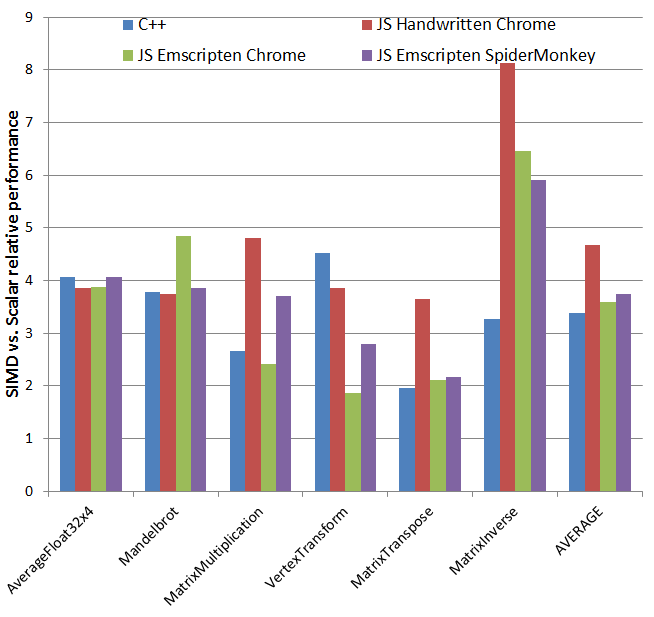
\includegraphics[width=0.45\textwidth]{figures/simd-scalar-speedup.png}
\end{center}
\caption{SIMD vs. Scalar relative speedups}
\label{fig:simd-scalar-speedup}
\end{figure}

\subsection{Scalar C++ vs. JavaScript}

Figure~\ref{fig:cpp-js-scalar} shows the relative scalar C++ vs. JavaScript
performance for each of the four combinations. Less than 1 means that the 
JavaScript kernel ran that much slower than the corresponding C++ kernel.

\begin{figure}
\begin{center}
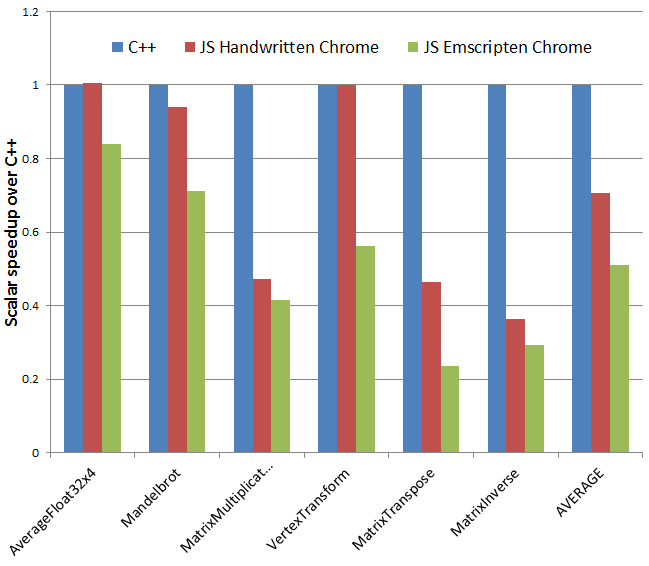
\includegraphics[width=0.45\textwidth]{figures/cpp-js-scalar.png}
\end{center}
\caption{Scalar C++ vs. Javascript relative performance}
\label{fig:cpp-js-scalar}
\end{figure}

\subsection{SIMD C++ vs. JavaScript}

Figure~\ref{fig:cpp-js-simd} shows the relative SIMD C++ vs. JavaScript
performance for each of the four combinations. Less than 1 means that the 
JavaScript kernel ran that much slower than the corresponding C++ kernel.

\begin{figure}
\begin{center}
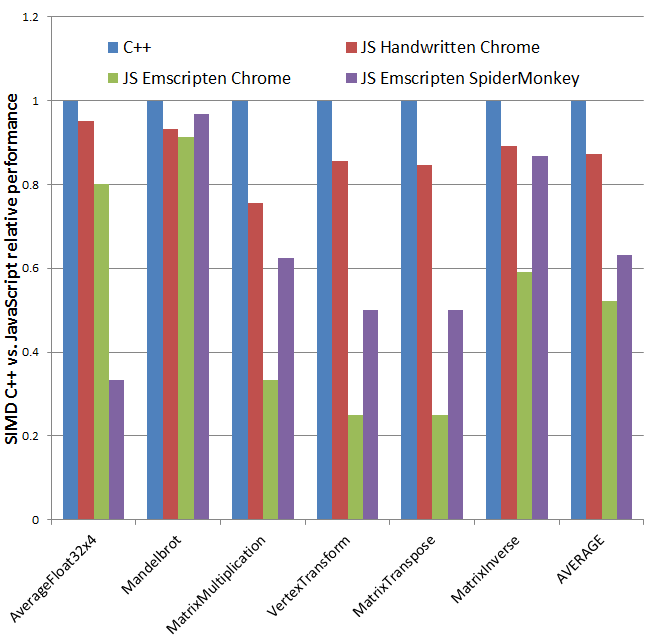
\includegraphics[width=0.45\textwidth]{figures/cpp-js-simd.png}
\end{center}
\caption{SIMD C++ vs. Javascript relative performance}
\label{fig:cpp-js-simd}
\end{figure}

\section{Summary}

\appendix
\section{Appendix Title}

This is the text of the appendix, if you need one.

\acks

Acknowledgments, if needed.

% We recommend abbrvnat bibliography style.

\bibliographystyle{abbrvnat}

% The bibliography should be embedded for final submission.

\begin{thebibliography}{}
\softraggedright

\bibitem[Smith et~al.(2009)Smith, Jones]{smith02}
P. Q. Smith, and X. Y. Jones. ...reference text...

\end{thebibliography}


\end{document}

%                       Revision History
%                       -------- -------
%  Date         Person  Ver.    Change
%  ----         ------  ----    ------

%  2013.06.29   TU      0.1--4  comments on permission/copyright notices

